\subsubsection{Zeeman Effect}
\label{toc:ZeemanEffect}
The Zeeman effect describes the separation of degenerated energy states in a static magnetic field. 
Dependent on the strength of the field, one distinguishes between three forms.
\begin{itemize}
	\item \textbf{Normal Zeeman Effect}\\
	The normal Zeeman effect is a special case of the anomalous Zeeman effect with a total spin equal to zero. The splitted energy leves are equidistant.
	\item \textbf{Anomalous Zeeman Effect}\\
	The anomalous Zeeman effect is the general case with a total spin unequal to zero. The splitting of the energy levels is hereby dependent on the quantum numbers $j$ and $l$.
	\item \textbf{Paschen-Back Effect}\\
	The Paschen-Back effect describes the case, in which the external magnetic field is much stronger than the internal one. 
This destroys the coupling between $\vec{L}$ and $\vec{S}$, so that each of them perform an independent precession around the external field's axis.
\end{itemize}
Lorentz introduced a semi classical theory without a spin.  
The electrons rotate on circular paths in the xy-plane and oszillate linearly in the z-plane. 
The magnetic moment due to the circular movement (refer to figure~\ref{fig:ElectronMagMom}) is given by
	\begin{align}
		\vec{\mu}_e = I\cdot \vec{A} = -e\nu \cdot \pi r^2 \hat{n} = -\frac{ev}{2\pi r}\cdot \pi r^2 \hat{n} = -\frac{e}{2m_e}\cdot \vec{L}\ .
	\end{align}

\begin{figure}[ht]
	\centering
	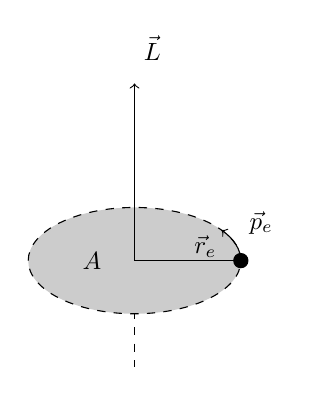
\begin{tikzpicture}[scale=0.9, transform shape]		
		\draw[dashed,black] (0,0) -- (0,-1.5);
		\draw[dashed,fill=black!20] (0,0) ellipse (1.5 and .75);
		\draw[black,->] (0,0) -- (0,2.5);	
		\draw[fill=black] (1.5,0) circle (0.1);
		\draw[black,->] (0,0) -- (1.5,0);
		\draw[black,->] (1.5,0) arc (0:35:1.5cm and 0.75cm);
		\node at (.25,3) {$\vec{L}$};
		\node [above right, black] at (1.5,.25) {$\vec{p}_e$};
		\node at (-.6,0) {$A$};
		\node at (1,0.2) {$\vec{r}_e$};
	\end{tikzpicture}
	\caption[Electron on a Circular Path]{Electron on a circular path with a magnetic moment $\vec{\mu}_e$}
	\label{fig:ElectronMagMom}
\end{figure}
With an external magnetic field $\vec{B}$ applied, the potential energy of a magnetic dipole with a momentum $\vec{\mu}$ is given by
	\begin{align}
		E_{\text{pot}} = -\vec{\mu}_e \cdot \vec{B} = \frac{e}{2m_e}\cdot \vec{L}\vec{B}\ .
	\label{eq:PotEnergyMagDipole}
	\end{align}
Assuming the magnetic field is parallel to the z direction $\vec{B} = (0,0,B)$, equation~\ref{eq:PotEnergyMagDipole} can be written as
	\begin{align}
		E_{\text{pot}} = \mu_{\text{B}} \cdot m \cdot B\ ,
	\end{align}
using $l_z = m\cdot \hbar$ and the Bohr magneton $\mu_{\text{B}} = \frac{e\hbar}{2m_e}$. 
Since $\Delta m = (0\ ,\pm 1)$ for transitions, there are three possible cases. 
$\Delta m = 0$ refers to the so called $\pi$-polarisation, the emitted light is linearly polarised. For $\Delta m = \pm 1$, the polaristion is called $\sigma^{\mp}$, the light is circularly polarised.
\begin{figure}[ht]
	\centering	
	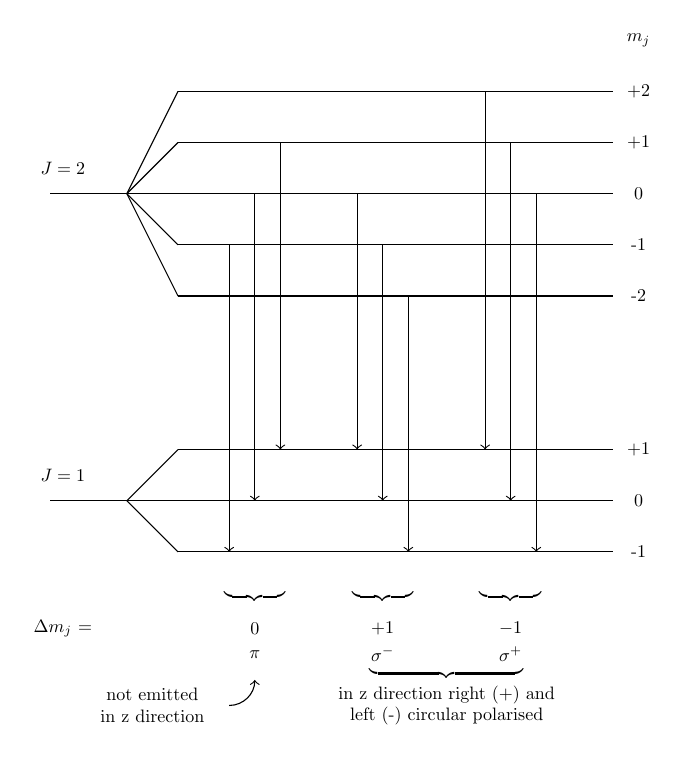
\begin{tikzpicture}[scale=0.65, transform shape]		
		% J = 2
		\node at (0.25,5.5) {$J = 2$};		

		\draw (0,5)	--	(11,5);
		\node at (11.5,5) {0};

		\draw (1.5,5)	--	(2.5,3);
		\draw (2.5,3)	--	(11,3);
		\node at (11.5,3) {-2};		

		\draw (1.5,5)	--	(2.5,4);
		\draw (2.5,4)	--	(11,4);
		\node at (11.5,4) {-1};
	
		\draw (1.5,5)	--	(2.5,6);
		\draw (2.5,6)	--	(11,6);
		\node at (11.5,6) {+1};		

		\draw (1.5,5)	--	(2.5,7);
		\draw (2.5,7)	--	(11,7);
		\node at (11.5,7) {+2};

		% J = 1
		\node at (0.25,-0.5) {$J = 1$};
			
		\draw (0,-1)	--	(11,-1);
		\node at (11.5,-1) {0};

		\draw (1.5,-1)	--	(2.5,-2);
		\draw (2.5,-2)	--	(11,-2);
		\node at (11.5,-2) {-1};

		\draw (1.5,-1)	--	(2.5,0);
		\draw (2.5,-0)	--	(11,-0);
		\node at (11.5,0) {+1};
		
		\node at (11.5,8) {$m_j$};
		
		\draw[->] (3.5,4)	--	(3.5,-2);
		\draw[->] (4.0,5)	--	(4.0,-1);
		\draw[->] (4.5,6)	--	(4.5,+0);

		\draw[->] (6.0,5)	--	(6.0,+0);
		\draw[->] (6.5,4)	--	(6.5,-1);
		\draw[->] (7.0,3)	--	(7.0,-2);
		
		\draw[->] (8.5,7)	--	(8.5,+0);
		\draw[->] (9.0,6)	--	(9.0,-1);
		\draw[->] (9.5,5)	--	(9.5,-2);

		\node at (4.0,-3)	{$\underbrace{\hspace{1.2cm}}_{}$};
		\node at (4.0,-3.5)	{$0$};
		\node at (4.0,-4)	{$\pi$};
		\node at (6.5,-3)	{$\underbrace{\hspace{1.2cm}}_{}$};
		\node at (6.5,-3.5)	{$+1$};
		\node at (6.5,-4)	{$\sigma^-$};
		\node at (9.0,-3)	{$\underbrace{\hspace{1.2cm}}_{}$};
		\node at (9.0,-3.5)	{$-1$};
		\node at (9.0,-4)	{$\sigma^+$};	

		\node [align=center] at (2,-5)	{not emitted\\in z direction};
		\draw [->] (3.5,-5) to [out=0,in=270] (4.0,-4.5);
	
		\node at (7.75,-4.5)	{$\underbrace{\hspace{3.0cm}}_{}$};
		\node [align=center] at (7.75,-5)	{in z direction right (+) and\\left (-) circular polarised}; 

		\node at (0.25,-3.5)	{$\Delta m_j$ =};
	\end{tikzpicture}
	\caption[Splitting of the Normal Zeeman Effect]{Splitting of the normal Zeeman effect. $\Delta m = 0$ results in linearly polarised light and $\Delta m = \pm 1$ yields $\sigma^{\mp}$ circular polarised light.}
	\label{fig:ZeemanSplitting}
\end{figure}\\
Another approach to the Zeeman effect is quantum mechanics. Using the magnetic moment and the spin moment of the electron
	\begin{align}
		\vec{\mu}_L = \frac{\mu_{\text{B}}}{\hbar}\vec{L} \hspace{1.0cm} \&\hspace{1.0cm} \vec{\mu}_S = g_s\frac{\mu_{\text{B}}}{\hbar}\vec{S}\ ,
	\end{align}
the total magnetic momentum $\vec{\mu}_J = \vec{\mu}_L + \vec{\mu}_S$ calculates to
	\begin{align}
		\vec{\mu}_J = -\frac{\mu_{\text{B}}}{\hbar}(\vec{L} + g_s\vec{S})\ ,
	\end{align}
where $g_s \approx 2$ is the electron spin g-factor. 
With help of perturbation theory one can calculate the eigenvalues of the Hamiltonian of the magnetic field 
	\begin{align}
	H_{\text{B}} = -\vec{\mu}_J \vec{B} = \frac{\mu_{\text{B}}}{\hbar}(\vec{J}+\vec{S})\vec{B}\ .
	\end{align}
The two magnetic moments interact with the magnetic field causing an energy level shift of
	\begin{align}
		\label{eq:ZeemanEnergyShift}
		\Delta E_{m_{j}} = m_j \cdot g_j \cdot \mu_{\text{B}}\cdot B\, \text{ with}\ g_j = 1 + \frac{j(j+1)+s(s+1)-l(l+1)}{2j(j+1)}
	\end{align}
referring to the Land\'{e} factor. 
For a total spin $s=0$ one gets $g_j = 1$, which represents the energy shift of the normal Zeeman effect. 
As for the classical approach there are rules for possible energy transitions
	\begin{align}
		\Delta m_j = 0 \mathrel{\widehat{=}} \pi \hspace{1.0cm} \& \hspace{1.0cm} \Delta m_j = \pm 1 \mathrel{\widehat{=}} \sigma^{\mp}\ ,
	\end{align}
that are shown in figure~\ref{fig:ZeemanSplitting}.
